\chapter[Introdução]{Introdução}
\label{chap:introducao}
	
	Para esclarecer o entendimento do projeto, foi definido um Termo de Abertura do Projeto (TAP). Ele tem como objetivo definir, de forma clara, o que é o projeto e quais são os seus limites. Neste capítulo estão registrados os tópicos do TAP para o projeto \textbf{Bancada de Teste de Amortecedores Veiculares}.

	\section{Definição do Problema}
	\label{sec:tap_problema}

		A tabela \ref{problema} apresenta de maneira compacta o problema central a ser solucionado com esse projeto, assim como os efeitos de uma solução bem sucedida.

		\begin{table}[h]
			\centering
			\caption{Descrição do problema}
			\label{problema}
			\resizebox{\textwidth}{!}{%
			\begin{tabular}{|
			>{\columncolor[HTML]{C0C0C0}}c |l|}
			\hline
			{\color[HTML]{000000} \textbf{O problema de}} & {\color[HTML]{000000} \begin{tabular}[c]{@{}l@{}}Dificuldade de obter de forma práticas as seguintes\\ informações: gráfico de força por velocidade que fornece\\ o coeficiente de amortecedor e a temperatura, as quais são\\ necessárias para caracterizar o amortecedor e auxiliar em\\ projeto de suspensão automotivas.\end{tabular}} \\ \hline
			{\color[HTML]{000000} \textbf{Afeta}} & {\color[HTML]{000000} \begin{tabular}[c]{@{}l@{}}O dimensionamento da suspensão e consequentemente\\ o conforto e estabilidade do veículo.\end{tabular}} \\ \hline
			{\color[HTML]{000000} \textbf{Cujo impacto}} & {\color[HTML]{000000} \begin{tabular}[c]{@{}l@{}}Aumento de custo do projeto e a redução da segurança\\ do veículo.\end{tabular}} \\ \hline
			{\color[HTML]{000000} \textbf{Os benefícios de uma solução seriam}} & {\color[HTML]{000000} \begin{tabular}[c]{@{}l@{}}Com as informações fornecidas pela bancada, seria possível\\ dimensionar o projeto de suspensão do veiculo de forma mais\\ precisa, aumentado a segurança deste. Com a obtenção do\\ gráfico gerado, será possível evidenciar as caraterísticas do\\ amortecedor oferecendo evidências empíricas ao usuário da\\ bancada.\end{tabular}} \\ \hline
			\end{tabular}%
			}
		\end{table}


	\section{Justificativa}
	\label{sec:tap_justificativa}

		Amortecedores veiculares têm por finalidade o controle de oscilações da suspensão, proporcionando estabilidade da carroceria, mantendo o contato da roda com o solo, assegurando maior conforto e segurança aos ocupantes do veículo. Logo, os amortecedores são componentes de suma importância em qualquer sistema veicular no qual se deseja atenuar vibrações \cite{Duarte}. Durante a fabricação de amortecedores faz-se necessária à utilização de um maquinário que seja capaz de testá-los e validá-los. A construção de um maquinário dessa natureza é extremamente importante e requerida, tanto para a indústria, quanto para fins acadêmicos e educativos.

		Estudiosos e empreendedores autônomos que atuam no ramo da suspensão veicular podem ter dificuldades para investir em maquinários de alto custo. Porém, muitas vezes necessitam de informações sobre comportamento do amortecedor em determinadas condições, como por exemplo, os gráficos de desempenho de amortecedores e a constante de amortecimento.

		Equipes de competições universitárias de Engenharia Automotiva existentes na UnB-FGA trabalham em projetos de suspensão de veículos para competições e necessitam de testes mais elaborados para que seus veículos se destaquem. Para estas equipes, a disponibilidade de uma bancada deste seguimento é muito desejável, tanto na etapa de projeto quanto na etapa de testes na fabricação de amortecedores.

		Cabe ressaltar que, para definir o amortecedor para determinado veículo, esta bancada pode ser um artifício determinante nesta escolha. A bancada poderá atuar na avaliação para escolha entre os amortecedores disponíveis. No âmbito acadêmico, uma bancada como a proposta no presente trabalho, pode mostrar-se de grande utilidade, pois possibilitaria ao estudante associar a prática aos conhecimentos teóricos adquiridos na universidade.

	\section{Objetivo Geral}
	\label{sec:tap_objetivo_geral}

		O objetivo geral do projeto é a criação de uma bancada para teste de amortecedores, para veículos leves de quatro rodas, visando o melhor entendimento sobre o seu funcionamento. Para isso, faz-se necessário a caracterização do amortecedor, a qual é composta por características geométricas, pela força atuante e outros fatores que influenciam seu funcionamento.
			

	\section{Objetivos Específicos}
	\label{sec:tap_objetivos_especificos}

		\begin{itemize}
			\item Criação de um projeto mecânico contendo as indicações dos componentes das peças para a montagem da bancada, bem como sua modelagem conceitual;
			\item Criação de um programa de interface humano-computador capaz de receber, processar, armazenar e apresentar dados e resultados relevantes ao experimento, tais como velocidade, deslocamento, entre outras definições relatadas posteriormente;
			\item Obtenção das características do amortecedor a partir dos testes realizados pela bancada;
			\item Elaboração de um manual de utilização da bancada contemplando as principais funcionalidades, dificuldades e forma de utilização;
			\item Apresentação de um relatório de características do amortecedor gerado a partir dos dados extraído do sensoriamento e comparação com curvas conhecidas na literatura;
			\item Preparação de um relatório do trabalho realizado, isto é, do projeto proposto, bem como todos os pontos abrangidos e negligenciados para construção da bancada.
		\end{itemize}
		

	\section{EAP}
	\label{sec:tap_EAP}

		A Estrutura Analítica do Projeto (EAP) é uma técnica de decomposição que consegue dividir os principais produtos do projeto em etapas que detalham o projeto com o intuito de auxiliar a equipe de gerenciamento na definição das atividades. A EAP do projeto é apresentada na Figura \ref{EAP}. Nas seções \ref{sec:tap_subprodutos} e \ref{sec:tap_lista} são listadas as descrições e detalhamentos dos pacotes de trabalho, de acordo com a EAP, e as definições do que \textit{é} e \textit{não é} entregável no projeto.

		\begin{figure}[!h]
			\centering
			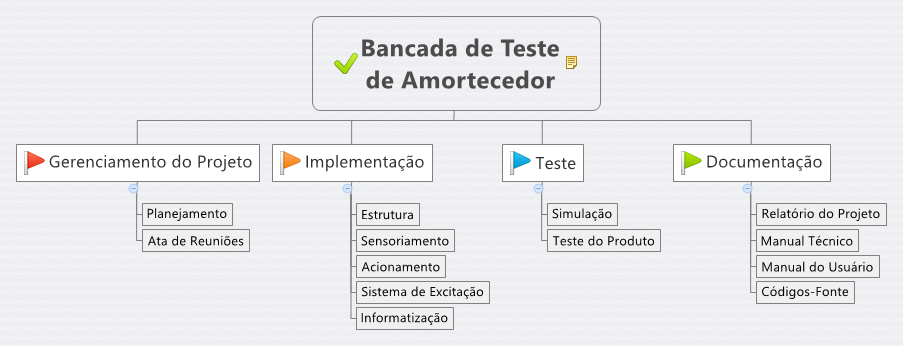
\includegraphics[scale=0.5]{EAPgeral.png}
			\caption{Estrutura Analítica Geral do Projeto}
			\label{EAP}
		\end{figure}


	\section{Descrição dos Subprotudos}
	\label{sec:tap_subprodutos}

		Nos parágrafos a seguir descreve-se brevemente os pacotes de trabalho apresentados na EAP Geral. 

		\textit{Gerenciamento do projeto}:
		Compreende um conjunto de ações que visa o planejamento e monitoramento da execução do projeto.

		\begin{itemize}
			\item{Planejamento}: Trata-se de esquematizar tarefas e prazos para execução.
			\item{Reuniões}: Refere-se ao acompanhamento do andamento da execução das atividades.
		\end{itemize}

		\textit{Documentação}:
		Envolve o conjunto de documentos a serem gerados durante o desenvolvimento do projeto.

		\begin{itemize}
			\item Relatório do Projeto: Trata-se do relatório que contém todas as informações pertinentes ao planejamento, pesquisa e execução.
			\item Manual Técnico: Documento a ser gerado ao final do projeto a fim de informar ao usuário todas as questões pertinentes à aplicabilidade bem como as limitações da bancada.
			\item Manual do Usuário: Documento a ser gerado ao final do projeto a fim de informar ao usuário o procedimento para execução do teste.
			\item Arquivo do Projeto: Arquivo digital contendo os códigos e simulações desenvolvidos.
		\end{itemize}

		\textit{Implementação}:
		Compreende efetivamente o processo de construção da bancada de teste de amortecedores.

		\begin{itemize}
			\item Estrutura: Trata-se da montagem da estrutura que sustenta os componentes da bancada.
			\item Sensoriamento: Sistema de aquisição dos dados obtidos por meio dos sensores de força, velocidade e temperatura.
			\item Acionamento: Sistema elétrico do acionamento do motor.
			\item Sistema de Exitação: Trata-se de um sistema biela manivela, necessário para transformação da velocidade angular em linear.
			\item Informatização: Sistema de tratamento para a entrada dos dados informados pelo usuário e apresentação dos resultados dos testes.
		\end{itemize}

		\textit{Testes}:
		Abrange o conjunto de testes realizados durante e após a construção da bancada.

		\begin{itemize}
			\item Teste do Produto: Teste realizado para verificar o funcionamento final da bancada.
		\end{itemize}


	\section{Lista É / Não É}
	\label{sec:tap_lista}

		\textbf{ É função do projeto:}

		\begin{itemize}
			\item Realizar a aquisição de todos os componentes necessários a montagem da bancada.
			\item Desenvolver aplicação web para interfaceamento dos resultados do teste.
			\item Implementar central de controle do teste.
			\item Realizar o interfaceamento dos componentes eletrônicos com o inversor de frequência.
			\item Idealizar e modelar a estrutura da bancada.
			\item Realizar simulação do mecanismo Biela-Manivela.
			\item Montar o mecanismo Biela-Manivela.
			\item Realizar testes do motor com e sem carga.
			\item Integrar os componentes na montagem final da bancada.
			\item Realizar rotinas de ajustes físicos e calibragem.
			\item Equacionar o sistema de transmissão.
		\end{itemize}

		\textbf{ Não é função do projeto:}

		\begin{itemize}
			\item Desenvolver o sistema de testes de suspensão.
			\item Desenvolver o sistema de testes com molas.
			\item Desenvolver um sistema com variação de perfil de pista.
			\item Desenvolver um sistema que opere fora das premissas definidas.
			\item Proporcionar ao usuário alterar o teste enquanto o mesmo estiver sendo executado.
			\item Realizar alteração do curso do amortecedor durante a execução do teste.
		\end{itemize}


	\section{Requisitos Preliminares}
	\label{sec:tap_requisitos}

		Os requisitos definem as condições de partida do projeto, alinhando os objetivos do mesmo com todas as partes interessadas. A seguir são apresentados os requisitos identificados para o sucesso do trabalho.

		\begin{itemize}
			\item A caracterização do amortecedor deverá se aproximar o máximo da realidade de funcionamento.
			\item As características do amortecedor deverão ser dimensionais, quanto a força e outros fatores, como temperatura.
			\item Para que o dimensionamento das peças e a definição das dimensões sejam projetados, deverá ser simulado - estaticamente e dinamicamente - o comportamento do sistema proposto, e a partir dessas simulações e aplicação, a escolha do tipo de material e o processo utilizado na fabricação.
			\item O sistema deverá contemplar uma interface interativa com o usuário, proporcionando a ele comodidade durante a realização do experimento, a partir da entrada de dados e geração do relatório final da experiência
			\item O teste deverá ser não destrutivo.
			\item A bancada será projetada para realizar testes de amortecedores com cursos de 100mm, 125mm e 150mm.
			\item A bancada será projetada para realizar testes para temperaturas entre 10$^{\circ}C$ e 120$^{\circ}C$.
			\item Os amortecedores deverão ser do tipo hidráulico.
			\item Os amortecedores deverão ser de veículos com peso bruto máximo de 1600 Kg.
			\item A faixa de variação da velocidade da haste é entre 175mm/s e 225mm/s, que são respectivamente 679,54 rpm e 1350 rpm no motor.
		\end{itemize}

		O detalhamento dos requisitos é abordado no tópico \nameref{chap:desenvolvimento} de acordo com a perspectiva de cada subárea.

	\section{Restrições}
	\label{sec:tap_riscos}

		As restrições definem condições limites para o projeto, apoiando decisões decorrentes do gerenciamento do produto e limitando o planejamento e desenvolvimento. Foram identificados como restrições os aspectos a seguir:

		\begin{itemize}
			\item \textbf{Custo}. Essa restrição ocorre pelo fato do projeto ser custeado pelo grupo desenvolvedor e está limitado a R\$: 200,00 (duzentos) reais por pessoa, como o grupo consiste em 11 (onze) integrantes, totaliza-se dois mil e duzentos reais.
			\item \textbf{Tempo}. Este projeto deve ser finalizado no dia 24 de junho de 2016. Essa data está alinhada com o período da disciplina de Projeto Integrador 2 (PI2). Logo, o planejamento e a execução do produto não devem exceder a esta data.
			\item \textbf{Deslocamento do Projeto}. Para a bancada proposta deve ser possível sua locomoção de acordo com necessidade, pois durante a apresentação dos pontos de controle ela deverá ser apresentada fisicamente, além de possibilitar os testes acordados.
			\item \textbf{Contextualização das Engenharias}. A bancada deve envolver abordagens das cinco engenharias envolvidas (eletrônica, software, aeroespacial, automotiva, energia). Assim, todos os membros do projeto poderão contribuir para solução final.
		\end{itemize}
